\documentclass[11pt]{article}

%%%%%%%%%%%%%%% PACKAGES %%%%%%%%%%%%%%%

\usepackage{url}
\usepackage{amssymb}
\usepackage{multicol}
\usepackage{enumerate}
\usepackage{tabularx}
\usepackage{graphicx}
\usepackage{amsmath}
\usepackage{amsfonts}
\usepackage{amsthm}
\usepackage{amscd}
\usepackage{amsrefs}
\usepackage[affil-it]{authblk}
\graphicspath{ {./images/} }

%%%%%%%%%%%%%%% TITLE/AUTHOR INFORMATION %%%%%%%%%%%%%%%

\title{The Art of Cryptography}
\author{Ismail Kably \& Duc Phan}
\date{\today}
\affil{Portland Community College}

%%%%%%%%%%%%%%% CUSTOM FORMAT %%%%%%%%%%%%%%%

\setlength{\textwidth}{6.5in}
\setlength{\textheight}{9in}
\setlength{\evensidemargin}{0in}
\setlength{\oddsidemargin}{0in}
\setlength{\topmargin}{+.4in}

\setlength{\oddsidemargin}{0.in}
\setlength{\evensidemargin}{0.in}
\setlength{\textwidth}{6.46in}
\setlength{\textheight}{8.4in}
\renewcommand{\abstractname}{Summary}

\usepackage{changepage}
\usepackage[margin=2.5cm]{geometry}

%%%%%%%%%%%%%%% PREAMBLE %%%%%%%%%%%%%%%

\newcommand{\Z}{\mathbb{Z}}
\newcommand{\Q}{\mathbb{Q}}
\newcommand{\R}{\mathbb{R}}
\newcommand{\C}{\mathbb{C}}
\newcommand{\norm}[1]{\left\lvert#1\right\rvert}    % Norm

%%%%%%%%%%%%%%% BEGIN DOCUMENT %%%%%%%%%%%%%%%

\begin{document}

\newenvironment{subs}
  {\adjustwidth{3em}{0pt}}
  {\endadjustwidth}
%%%%%%%%%%%%%%% TITLE %%%%%%%%%%%%%%%

\maketitle

%%%%%%%%%%%%%%% ABSTRACT %%%%%%%%%%%%%%%

\begin{abstract}

This paper seeks to discuss cryptography and how it works through some examples

\end{abstract}

%%%%%%%%%%%%%%% BODY OF PAPER %%%%%%%%%%%%%%%
\section{What is cryptography?}
\phantom{x}\hspace{3mm}Cryptography or cryptology is the practice and study of techniques for secure communication in the presence of third parties called adversaries. Cryptography is associated with the process of converting ordinary plain text into unintelligible text and vice-versa. It is a method of storing and transmitting data in a particular form so that only those for whom it is intended can read and process it. \\
\phantom{x}\hspace{3mm}Cryptography not only protects data from theft or alteration, but can also be used for user authentication. More generally, cryptography is about constructing and analyzing protocols that prevent third parties or the public from reading private messages.\\


\section{Why Linear Algebra?}
\phantom{x}\hspace{3mm}Cryptography exists in many forms, some use Number Theories, some use Linear Algebra. However, because the type of encryption discussed in this paper use the Math behind matrices, the knowledge of Linear Algebra is required.\\
\phantom{x}\hspace{3mm}Even though the algorithms to implement encryption can become very complicated, the general idea is easy to understand. Cryptography can as simple as using a 3x3 matrix composed of random	integers that represent the characters in the plain-text to encrypt the text.
\pagebreak

\section{A simple example of Encryption}
\phantom{x}\hspace{3mm}In this example, we will try to encrypt the word ''MATH.'' There are various ways to achieve the goal, but this example, we will use a very simple type of cryptography.\\
\phantom{x}\hspace{1mm}The process consists of three steps:

\begin{enumerate}[1.]
\addtolength{\itemindent}{20mm}
	\item Convert the word ''MATH'' into a plain-text matrix.
	\item Encrypt the plain-text matrix.
	\item Decrypt the encrypted matrix.
\end{enumerate}

\begin{subs}
\subsection{Conversion}
\phantom{x}\hspace{3mm}Each character in plain-text must be denoted with a numerical value and placed into a matrix. The numerical rules can vary as long as they are consistent throughout the process.\\\\
\phantom{x}\hspace{1mm}In this example, we will use the numerical rule shown below:\vspace{3mm}
\begin{center}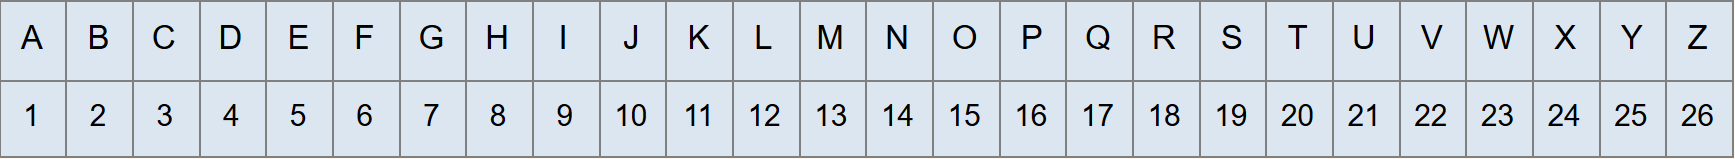
\includegraphics[scale=0.275]{numerical}\vspace{5mm}\end{center}

First, each letter will be used as entries of vectors to put into the matrix, such that:
	\begin{enumerate}
	\itemsep-1em 
	\item The number of entries of each vector is equivalent to the number of rows of the cipher matrix (which will be discusses later).\\
	\item Letters are placed one at a time, going down a row for each value.\\
	\item Vectors are filled one to another.\\
	\item The remaining empty entries in the last vector is filled with space.\vspace{3mm}
	\end{enumerate}
Afterward, the characters in the vectors are then converted into their corresponding numerical values using the rule above.
\begin{center} 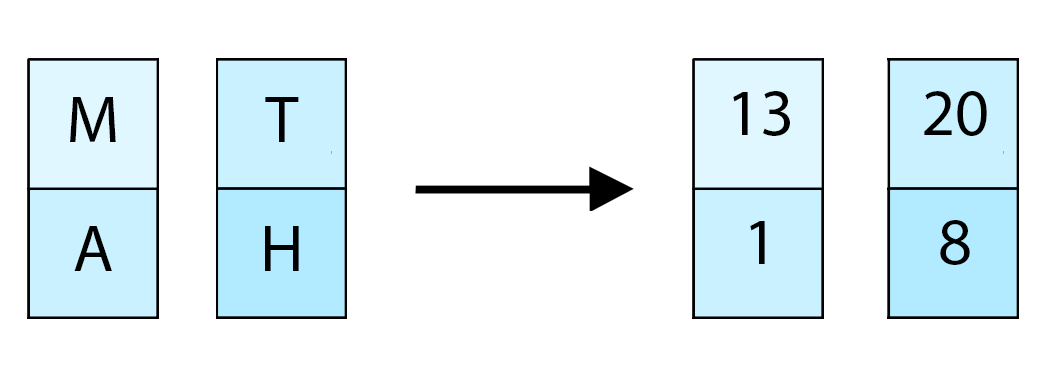
\includegraphics[scale=0.2]{math_1} \end{center}

Finally, the vectors are augmented to form the plain-text matrix.
\begin{center} 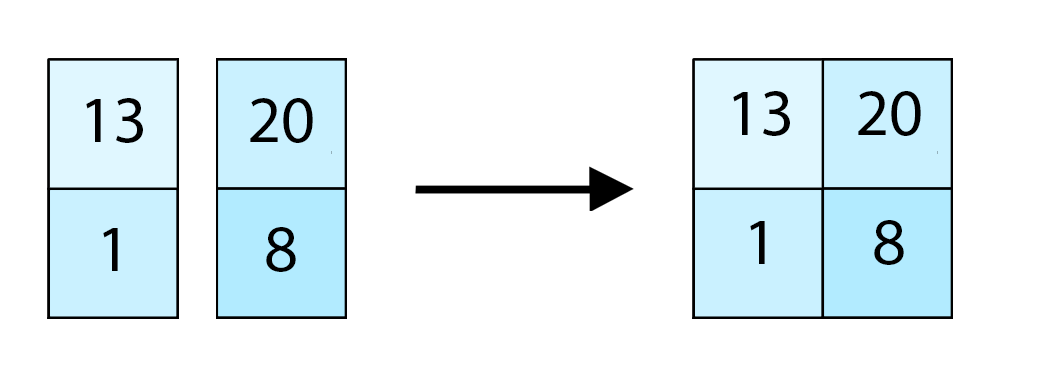
\includegraphics[scale=0.2]{MATH} \end{center}
\pagebreak

\subsection{Encryption}
In this method, we will use a matrix called cipher-matrix for the encryption step.\\The cipher matrix's values can be randomly generated as long as it is invertible, but its size is fixed beforehand.\vspace{5mm}\\
To make it easy, we will use a 2x2 matrix.\\The cipher matrix will then be used to multiply with the plain-text matrix as shown below:
\begin{center} 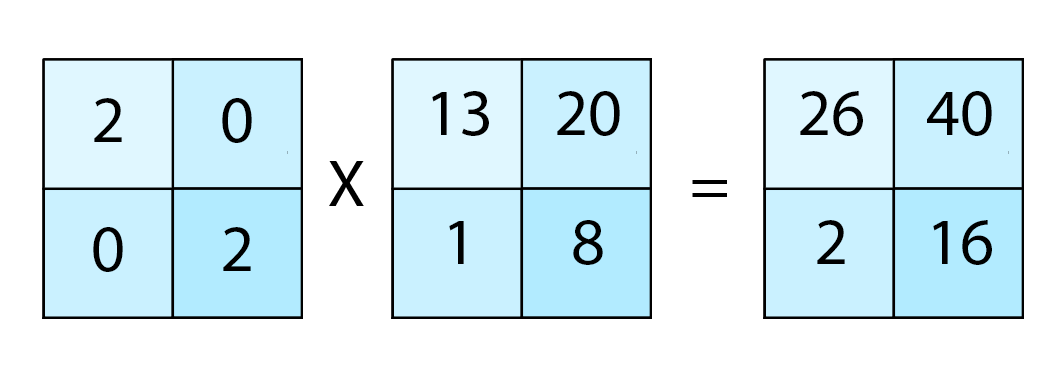
\includegraphics[scale=0.2]{multiply_1} \end{center}\vspace{5mm}
We can keep adding more steps for the encryption process to enhance the security, but doing so will greatly increase the complexity of the algorithm with the cost of performance.\\
To keep it simple, we'll stop in this step for this example. Thus, the product is called the encrypted matrix.

\subsection{Decryption}
After the encryption is completed, the encrypted and the cipher matrix will be sent to the recipient. In order to read the message, the recipient needs to go through the process of decryption, which - in this case - will be the encryption process in reverse. Since the sending process is out of topic, it will not be discussed in this paper.\vspace{5mm}\\
Let's take a look at this logic: 
	\begin{align*}
		& &&C \times P &&&= \phantom{xxxxx} E\\
		&\iff &&C^{-1} \times C \times P &&&= C^{-1} \times E\\
		&\iff &&P &&&= C^{-1} \times E
	\end{align*}
\phantom{x}\hspace{3mm}where C is the cipher matrix, P is the plain-text matrix and E is the encrypted matrix.\vspace{3mm}\\
Because the encrypted matrix was found using the multiplication between the cipher matrix and the plain-text matrix where the cipher matrix is on the left side of the plain-text matrix - since the recipient is given the cipher matrix and the encrypted matrix - the plain-text matrix can be found using the multiplication of the inverse of the cipher matrix and the encrypted matrix.\vspace{3mm}\\
\pagebreak

First, we can find the inverse using the sledgehammer given by our teacher, Mr. Damien!\\
\begin{center} 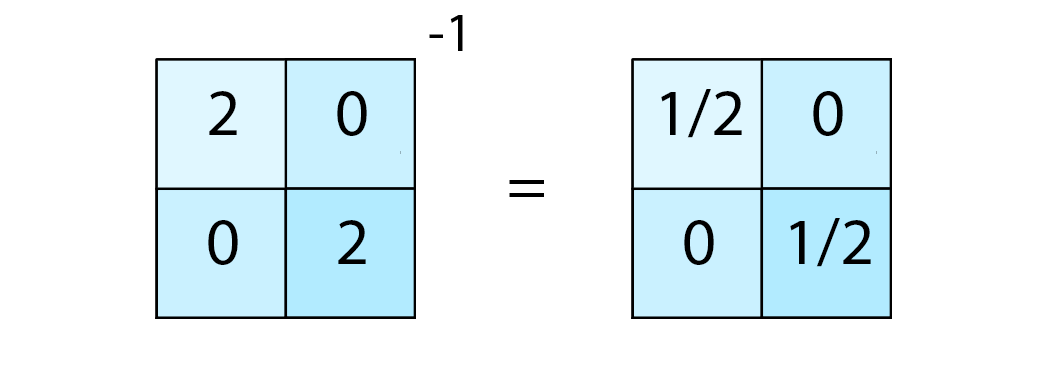
\includegraphics[scale=0.2]{inverse_1} \end{center}\vspace{5mm}

The inverted matrix is then multiplied with the cipher-text matrix (which will be on the left side). The product is the original plain-text matrix.
\begin{center} 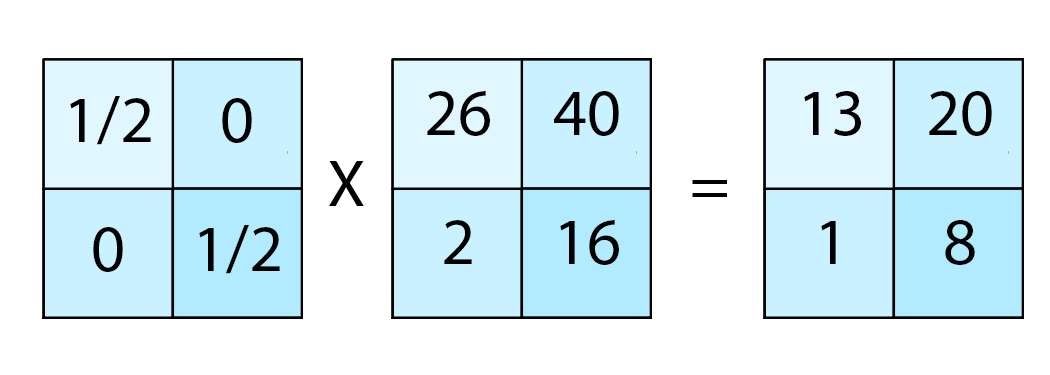
\includegraphics[scale=0.2]{multiply_2} \end{center}\vspace{5mm}

Afterward, we need to convert the matrix into the original message.\\
First, we need to split the columns of the decrypted matrix into vectors.
\begin{center} \includegraphics[scale=0.2]{linear_2} \end{center}\vspace{5mm}
Then, using the same numerical values to convert each character into the original message vectors.
\begin{center} 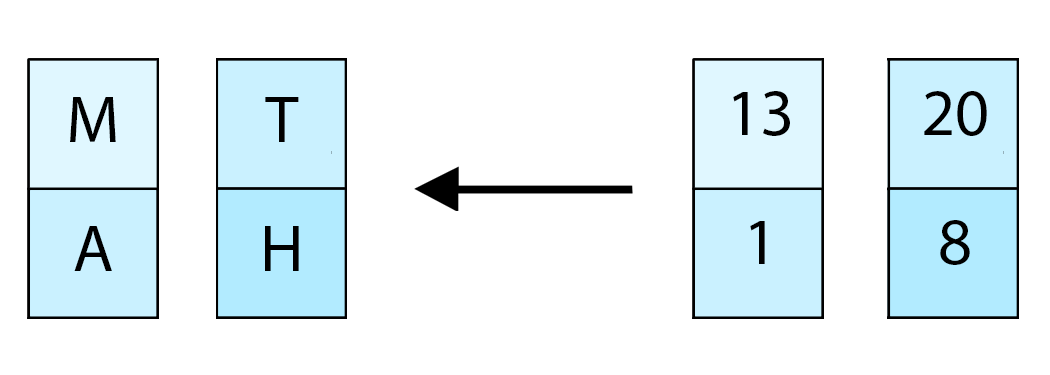
\includegraphics[scale=0.2]{math_2} \end{center}\vspace{5mm}
\begin{center} 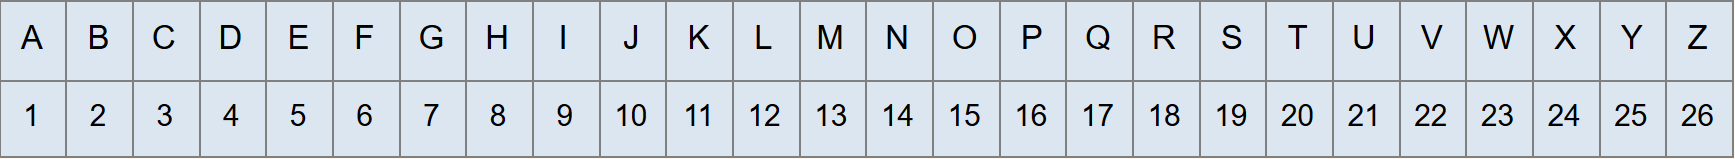
\includegraphics[scale=0.35]{numerical} \end{center}\vspace{5mm}

Each character in the vectors are then taken out to form the original message, from left to right, from top to bottom.\vspace{10mm}\\
Finally, we successfully decrypt the word ''MATH''!
\end{subs}

%%%%%%%%%%%%%%% BIBLIOGRAPHY %%%%%%%%%%%%%%%

\begin{bibdiv}
\begin{biblist}

%If you cite a book, here is how to cite

 \bib{A}{book}{
  title = {Write the title of the book here},
  author = {Write the author of the book here},
  publisher = {Write the publisher of the book here},
  date = {Write the year the book was published here},
  page = {If you cite a particular page number, or several pages, include them here}
 }
 
 \bib{B}{book}{
  title = {If you use another book, do the same thing as before},
  author = {etc.}
 }
 https://economictimes.indiatimes.com/definition/cryptography
 
\end{biblist}
\end{bibdiv}

%%%%%%%%%%%%%%% END DOCUMENT %%%%%%%%%%%%%%%

\end{document}